% File: Igloo.tex
% Author: Adam Leeper
%------------------------------------------------------------------------------
\providecommand{\isolatedBuild}[1]{#1}% Fallback definition to build normally.
\isolatedBuild{
  \documentclass[11pt,letterpaper]{book}
  %\documentclass[11pt,letterpaper]{book}

% aleeper: I think these are needed for Paul's macros?
\usepackage{epsfig}
\usepackage{epstopdf}

%\makeatletter
%\typeout{The import path is \import@path}
%\makeatother

\usepackage{import}

\subimport{./}{packagesMitiguy.sty}
\subimport{./}{macrosMitiguy.tex}
\subimport{./}{PageStylesMitiguy.tex}
\subimport{./}{macrosLeeper.tex}
   % Found via TEXINPUTS environment variable.
  \isolatedBuildHeader{Forces and Acceleration in Circular Motion}
                      {Forces and Acceleration in Circular Motion}
}
%%%
%%%
%%%
\begin{minipage}{0.5\linewidth}
  The figure shows a particle $Q$, of mass $m^Q$, sliding on a semi-circular
  igloo (smooth and made of ice) of radius $R$. The igloo is fixed in a
  Newtonian reference frame $N$ and is centered at point $N_o$.
  Right-handed orthogonal unit vectors are assigned as shown.
  Assume the particle is released from rest near the top of the igloo.
\end{minipage}
%\hspace{0.5cm}
\begin{minipage}{0.4\textwidth}
  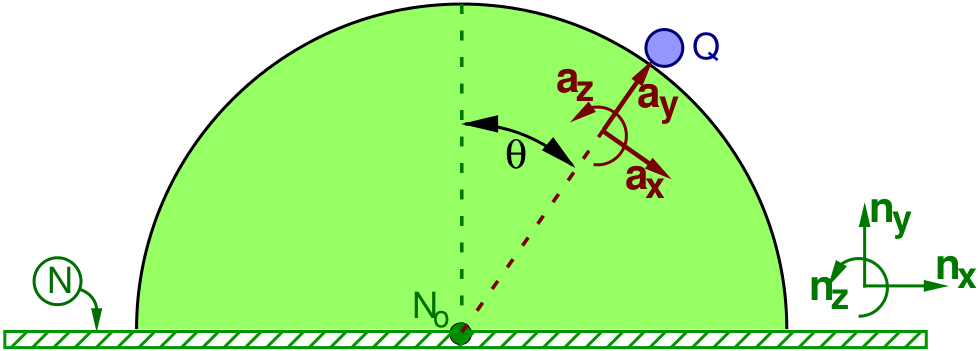
\includegraphics[width=9cm]{igloo.png}
\end{minipage}

\begin{enumerate}
  \item Use energy methods to obtain an expression for the speed of the
    particle as a function of $\theta$.
  \item Determine the value of $\theta$ when the particle loses contact with
    the the igloo.
    \\[0.0pc]\textbf{Hint:} Do a roadmap that helps you solve for the
    relevant contact force.
  \item Now assume the igloo is made of concrete, so a solid ball $B$ with
    mass $m^B = m^Q$ rolls down the igloo. Will the ball lose contact at a
    smaller, larger, or equal value of $\theta$? Explain your reasoning.
\end{enumerate}
%
\isolatedBuildFooter
